\documentclass[11pt]{article}
\usepackage{geometry}                % See geometry.pdf to learn the layout options. There are lots.
\geometry{letterpaper}                   % ... or a4paper or a5paper or ... 
%\geometry{landscape}                % Activate for for rotated page geometry
%\usepackage[parfill]{parskip}    % Activate to begin paragraphs with an empty line rather than an indent
\usepackage{graphicx}
\usepackage{amssymb}
\usepackage{amsmath}
\usepackage{epstopdf}
\usepackage{subfigure}
\usepackage[colorlinks=true, pdfstartview=FitV, linkcolor=black, citecolor=black, urlcolor=blue]{hyperref} % to be able to hyperlink to figures, etc, in text
\usepackage{natbib} % for better bibliography referencing. \citet without parentheses and \citep with them%
%\usepackage{fancyvrb} % This is to be able to make boxes around verbatim code in figures
% The following are to be able to go to smaller heading than subsubsection. Use "paragraph" and then "subparagraph"
\setcounter{secnumdepth}{5} % to be able to use more section headings
% here are the section headings in order to use in the text:
%\section{} % level 1
%\subsection{} % level 2
%\subsubsection{} % level 3
%\paragraph{} % level 4 - equivalent to subsubsubsection
%\subparagraph{} % level 5
%%%
\setcounter{tocdepth}{5} % To include all of the section headings in the table of contents
\DeclareGraphicsRule{.tif}{png}{.png}{`convert #1 `dirname #1`/`basename #1 .tif`.png}

\title{Oil Tracking on the TX-LA Shelf}
\author{Kristen M. Thyng}
%%\date{January 27, 2011}                                           % Activate to display a given date or no date


% a few handy macros

\newcommand\matlab{{\sc matlab}}
\newcommand{\goto}{\rightarrow}
\newcommand{\bigo}{{\mathcal O}}
\newcommand{\half}{\frac{1}{2}}
%\newcommand\implies{\quad\Longrightarrow\quad}
\newcommand\reals{{{\rm l} \kern -.15em {\rm R} }}
\newcommand\complex{{\raisebox{.043ex}{\rule{0.07em}{1.56ex}} \hskip -.35em {\rm C}}}


% macros for matrices/vectors:

% matrix environment for vectors or matrices where elements are centered
\newenvironment{mat}{\left[\begin{array}{ccccccccccccccc}}{\end{array}\right]}
\newcommand\bcm{\begin{mat}}
\newcommand\ecm{\end{mat}}

% matrix environment for vectors or matrices where elements are right justifvied
\newenvironment{rmat}{\left[\begin{array}{rrrrrrrrrrrrr}}{\end{array}\right]}
\newcommand\brm{\begin{rmat}}
\newcommand\erm{\end{rmat}}

% for left brace and a set of choices
\newenvironment{choices}{\left\{ \begin{array}{ll}}{\end{array}\right.}
\newcommand\when{&\text{if~}}
\newcommand\otherwise{&\text{otherwise}}
% sample usage:
%  \delta_{ij} = \begin{choices} 1 \when i=j, \\ 0 \otherwise \end{choices}


% for labeling and referencing equations:
\newcommand{\eql}{\begin{equation}\label}
\newcommand{\eqn}[1]{(\ref{#1})}
% can then do
%  \eql{eqnlabel}
%  ...
%  \end{equation}
% and refer to it as equation \eqn{eqnlabel}.  


% some useful macros for finite difference methods:
\newcommand\unp{U^{n+1}}
\newcommand\unm{U^{n-1}}

% for chemical reactions:
\newcommand{\react}[1]{\stackrel{K_{#1}}{\rightarrow}}
\newcommand{\reactb}[2]{\stackrel{K_{#1}}{~\stackrel{\rightleftharpoons}
   {\scriptstyle K_{#2}}}~}

% Headers for exercises:

\newcommand{\exercise}[1]{\vskip 15pt  \noindent {\large \bf Exercise #1}%
     \nopagebreak\vskip 5pt \nopagebreak}

\newcommand{\chapexercises}[1]{%
     \cleardoublepage
     \centerline{\LARGE\bf Chapter #1 Exercises}
     \vskip .5cm
     \noindent
     From: {\it Finite Difference Methods for Ordinary and Partial 
     Differential Equations}\\  by R.~J.~LeVeque, SIAM, 2007.~~~
     {\tt http://www.amath.washington.edu/$\sim$rjl/fdmbook}
     \vskip .5cm
     }


%% Kristen's added
% Partial derivative d
\newcommand{\p}{\partial}
% integral dt
\newcommand{\dd}{\text{d}}
\newcommand{\ul}{\uvec{\ell}}
%\newcommand{\dx}{\text{dx}}
%\newcommand{\dy}{\text{dy}}
%\newcommand{\dr}{\text{dr}}
%\newcommand{\dl}{\text{d$\uvec{\ell}$}}
% Full partial derivative fraction, use like \pd[x]{t} for \frac{\partial x}{\partial t}
\newcommand{\pd[2]}{\frac{\partial #1}{\partial #2}}
% left and right big parentheses, \left{ and \right} as \lp and \rp
\newcommand{\lp}{\left(}
\newcommand{\rp}{\right)}
\newcommand{\uvec}{\underline} % for vectors
\newcommand{\uuvec[1]}{\underline{\underline #1 }} % for tensors
\newcommand{\ovec}{\overline} % for reynolds stresses

% Better tilde: http://tex.stackexchange.com/questions/9363/how-does-one-insert-a-backslash-or-a-tilde-into-latex
\newcommand{\ttilde}{{\raise.17ex\hbox{$\scriptstyle\sim$}}}

% \linenumbers % add line numbers

% \begin{frontmatter}

\begin{document}
\maketitle

\section{Introduction}

% Summarize literature on particle tracking, particularly applications of tracmass. Include potentially pitfalls and things to be aware of.
\subsection{Particle Tracking}


% How does the tracking code work in general?
\section{Tracking Algorithm Sensitivity and Details}

% Summarize tracmass and tracpy details
\subsection{Explain Algorithm}

\subsubsection{2D Boundaries}

Due to the basic algorithm of TRACMASS, at boundaries within the numerical domain, drifters will be stopped according to the bounding fluxes. For a given grid cell in the 2D case, there are four fluxes controlling a drifter's movement. Drifters have nonzero fluxes on active sides of the cell and zero fluxes along masked land. They can run along these walls but should not penetrate them. At open numerical boundaries, the drifters will be stopped according to a check built into tracmass itself, and will be left with their final position along the open boundary and a flag indicating that they have exited the domain so they will not be stepped forward.

The addition of subgrid turbulence parameterizations can affect this. One method is to add parameterized turbulent values to the fluxes used to calculate drifter movements. These do not affect the fact that fluxes will be zero at masked land because they are multiplied by the original ufluxes to get the fluctuation to add to the original flux values.

However, there are two methods of adding in a random walk to the particle positions directly, and these were affecting the boundary behavior of drifters near walls. The problem was that when a drifter was alongside a masked land cell, if the random new position of the drifter was just right to move the drifter from its current cell into the land cell, then an error check later in the code for the volume of the cell would catch the drifter (due to its cell having zero volume since it was on land) and the drifter would be stopped at its location near land. Since drifters in the advection-only and turbulent velocity methods do not hit land, the overall behavior was different along the coastline for the diffusion and anisodiffusion methods (in these methods, many more drifters were congregated alongshore). I changed this by adding a check in the diffusion subroutine in tracmass to not accept a new displacement location for a drifter if the layer thickness (dzt) of that new location is zero. Now, I think that all of the routines will have similar coastline behavior. If, on the other hand, it is desired that drifters should be able to hit the coastline and ``beach,'' then this behavior in the diffusion routines might be desired.

% Diffusion parameters and number of interpolation steps
\subsection{Examine Sensivity of Results to Input Parameters}

A series of numerical surface drifter experiments were run for 16 days forward in time from 11/20/2009 with several changing parameters to understand their importance to the results.

There is little overall difference for the number of time interpolation steps for these simulations (not shown).

The difference in the results from diffusion types is illustrated in Figure \ref{diffusiontype}. For numerical drifter experiments with drifters initially seeded 10 km apart and using the same horizontal diffusivity, the difference in tracks and final positions is not extreme, but is noticeable. The cases with no diffusion and parameterized turbulent velocities (Figures \ref{diffusiontype-none} and \ref{diffusiontype-turb}) are similar, though a larger value of $A_H$ would presumably change this more. The cases with a random walk-type diffusion added to the particle tracks themselves (Figures \ref{diffusiontype-aniso} and \ref{diffusiontype-diff}) show more diffused behavior and are fairly similar to each other.

\begin{figure}
	\centering
	\subfigure[No diffusion]{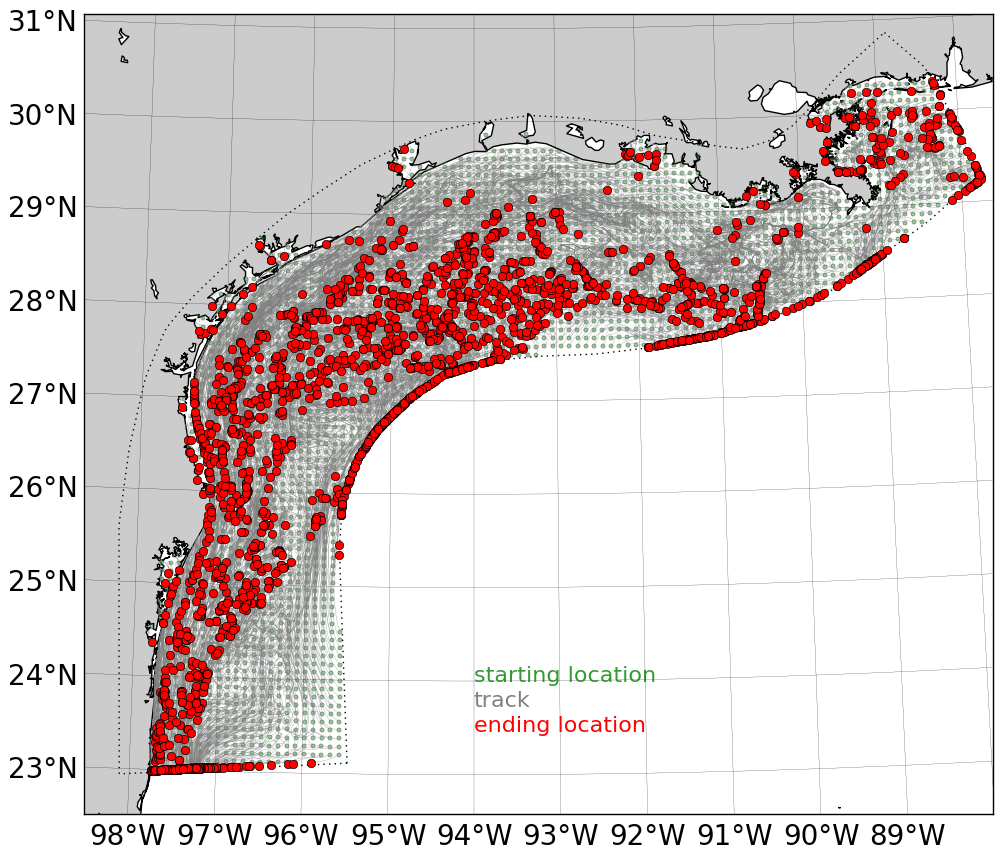
\includegraphics[width=.235\textwidth]{figures/10_5_None_Ftracks} \label{diffusiontype-none}}
	\subfigure[Turbulence]{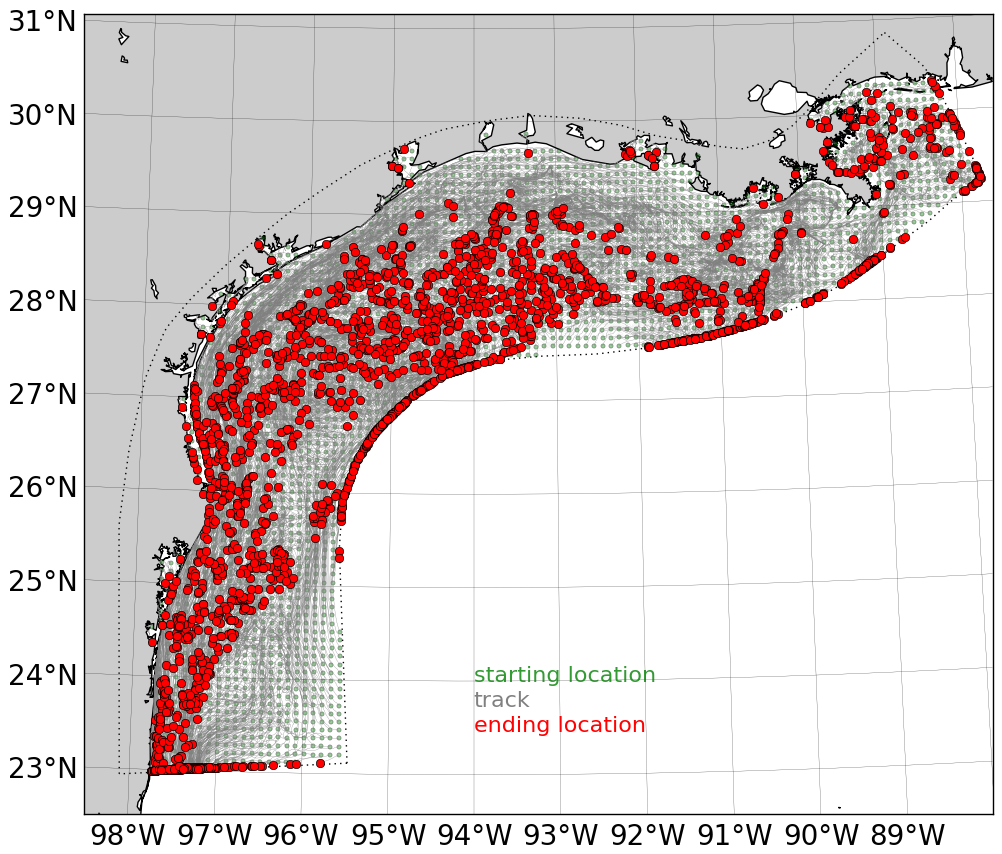
\includegraphics[width=.235\textwidth]{figures/10_5_Turb20_Ftracks} \label{diffusiontype-turb}}
	\subfigure[Elliptical]{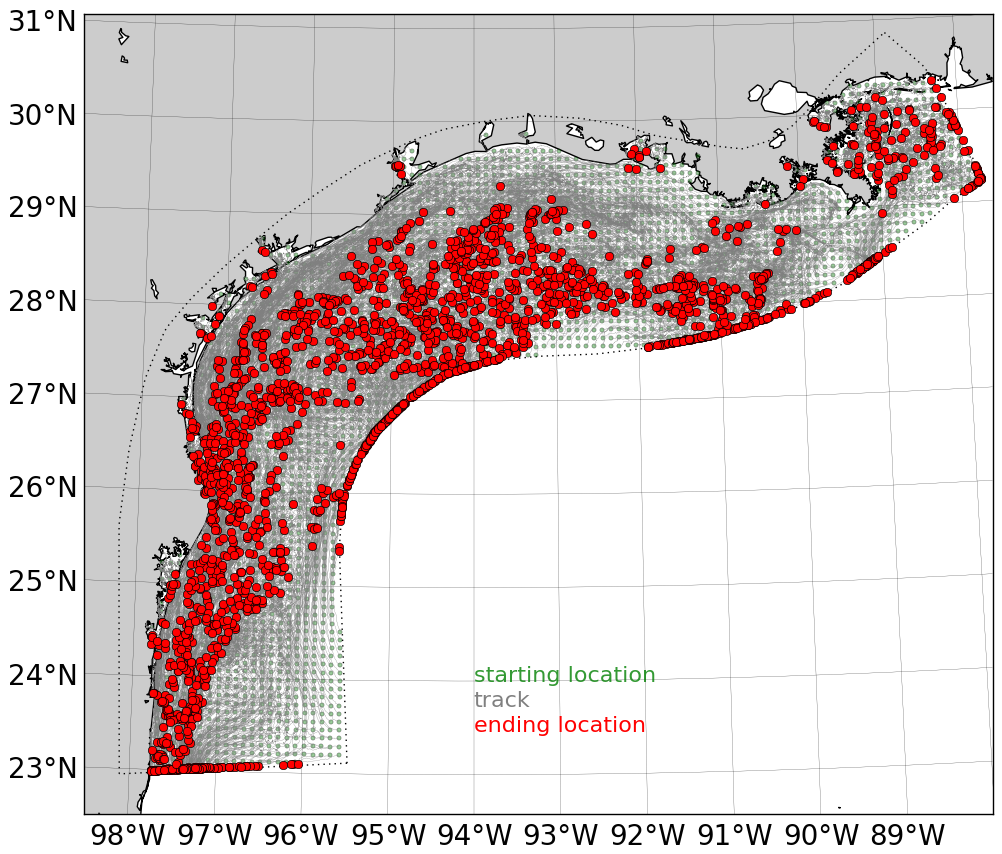
\includegraphics[width=.235\textwidth]{figures/10_5_A20_Ftracks} \label{diffusiontype-aniso}}
	\subfigure[Circular]{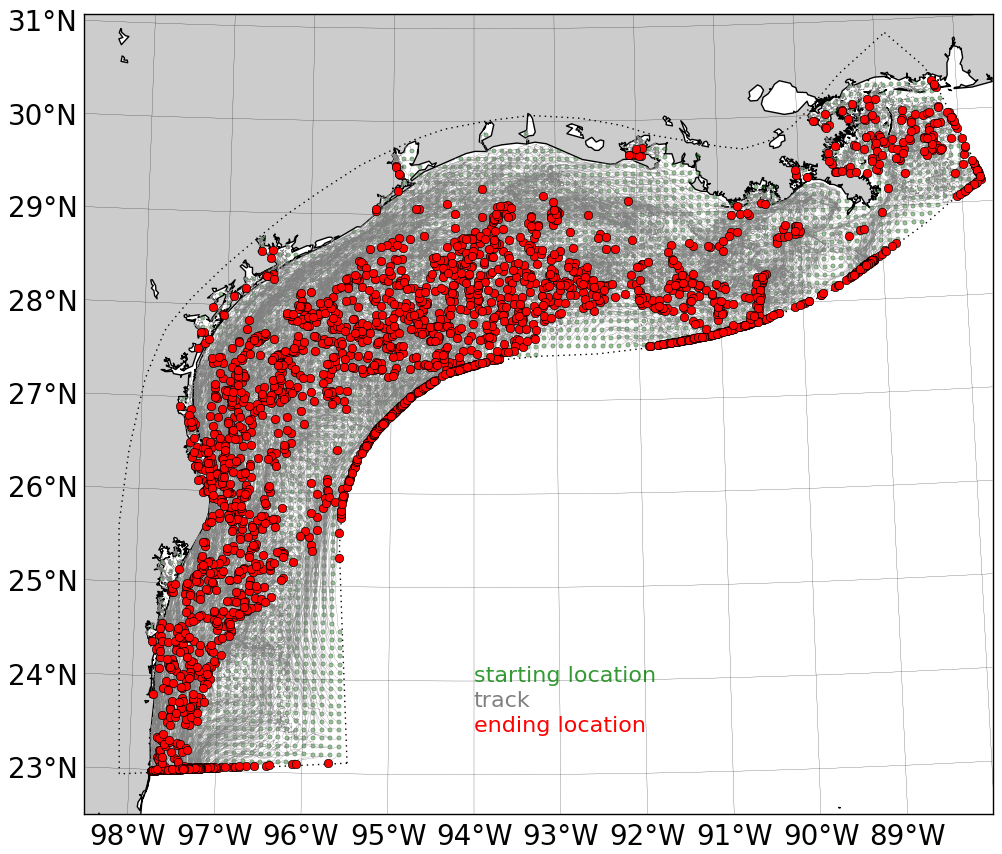
\includegraphics[width=.235\textwidth]{figures/10_5_D20_Ftracks} \label{diffusiontype-diff}}
	\caption{Comparison of types of diffusion for $A_H=20$ m$^2$/s, initial spacing of 10km}
	\label{diffusiontype}
\end{figure}


\begin{figure}
	\centering
	\subfigure[No diffusion]{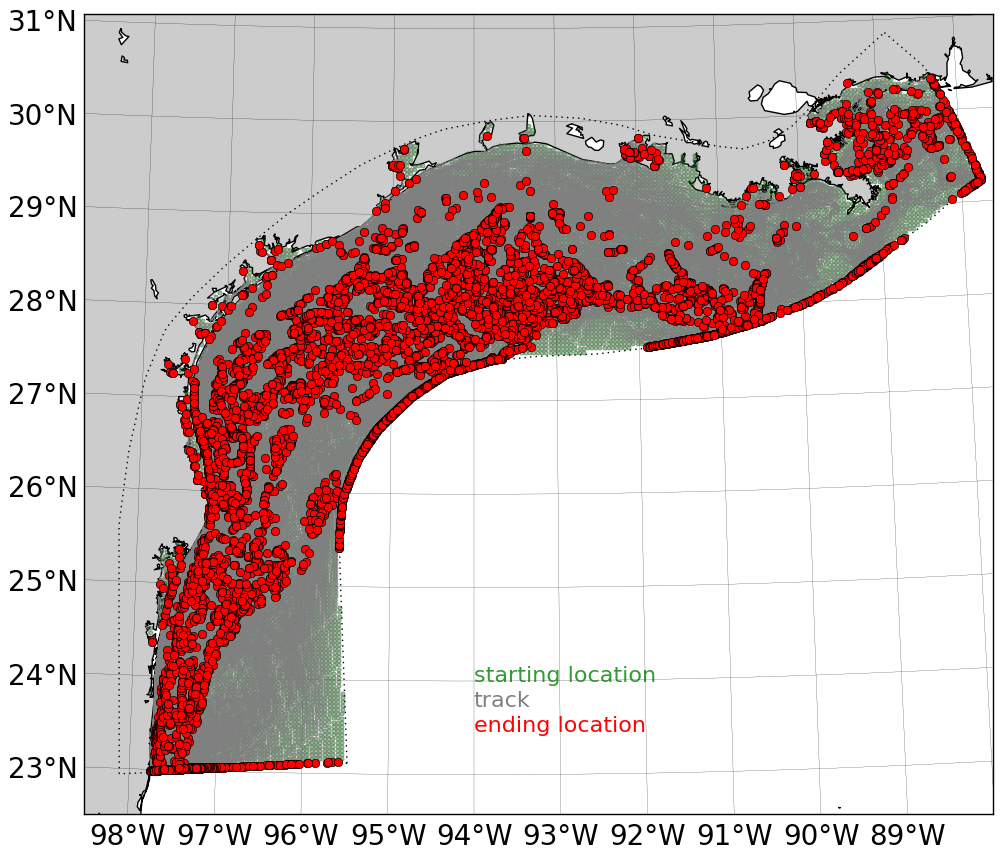
\includegraphics[width=.315\textwidth]{figures/5_5_None_Ftracks} \label{diffusionsize-none}}
	\subfigure[Circular diffusion, $A_H=5$]{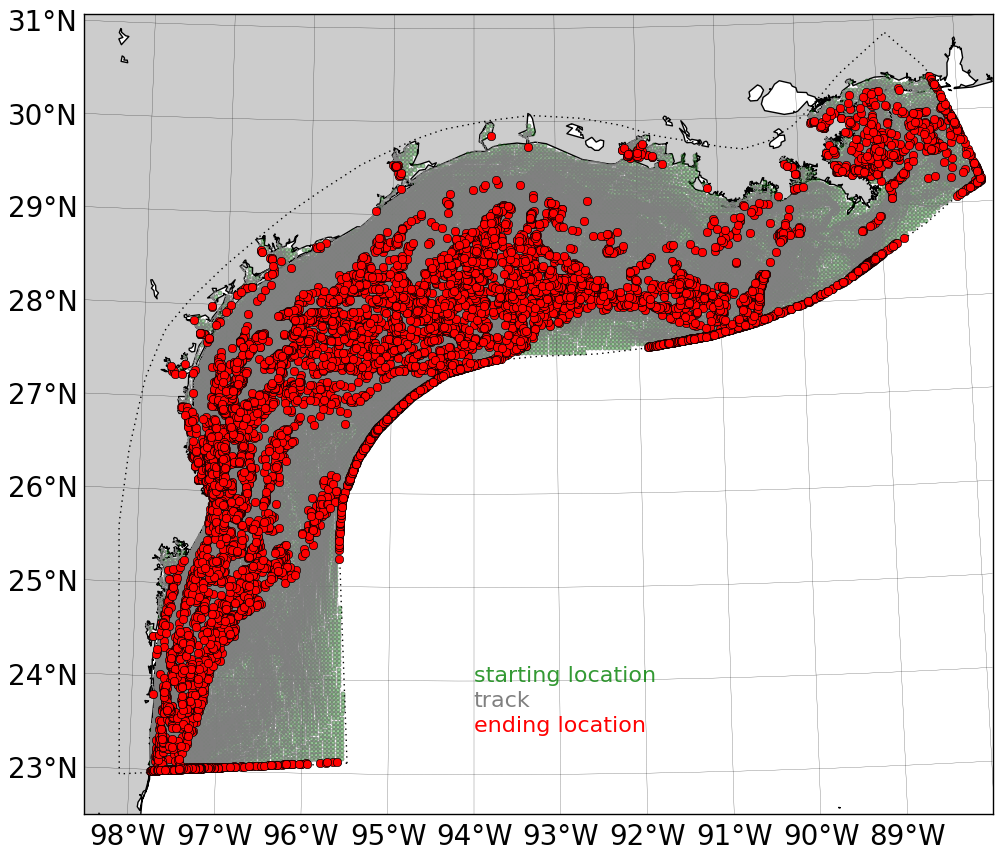
\includegraphics[width=.315\textwidth]{figures/5_5_D5_Ftracks} \label{diffusionsize-5}}
	\subfigure[Circular diffusion, $A_H=20$]{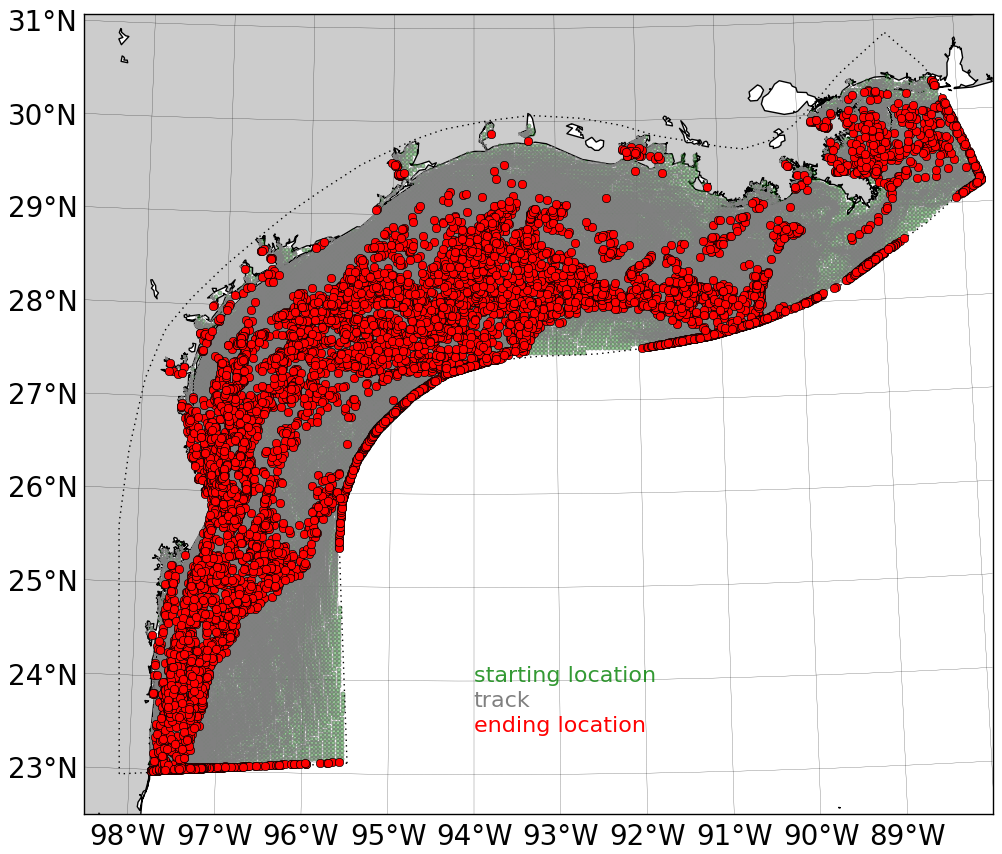
\includegraphics[width=.315\textwidth]{figures/5_5_D20_Ftracks} \label{diffusionsize-20}}
	\caption{Comparison of size of $A_H$ for initial spacing of 5km}
	\label{diffusionsize}
\end{figure}


\begin{figure}
	\centering
	\subfigure[Circular, 5 km spacing]{\includegraphics[width=.325\textwidth]{figures/5_5_D20_Fhistpcolor}}
	\subfigure[Circular, 10 km spacing]{\includegraphics[width=.325\textwidth]{figures/10_5_D20_Fhistpcolor}}
	\subfigure[Circular, 50 km spacing]{\includegraphics[width=.325\textwidth]{figures/50_5_D20_Fhistpcolor}}
	\caption{Comparison of initial drifter spacing with diffusion ($A_H=20$ m$^2$/s.}
\end{figure}

% \subsubsection{Number of Interpolation Steps}

% \subsubsection{Subgrid Turbulence Parameterizations}

% \paragraph{Turbulence}

% Read about and try some values of a

% \paragraph{Diffusion on a Circle}

% Vary parameters

% \paragraph{Diffusion on an Ellipse}

% Vary parameters

% Move drifters backward and forward from Galveston and compare
\subsection{Forward/Backward}


% How well does the particle tracking apply to the TXLA shelf?
\section{Performance of Model and Tracker}

% Can I recreate the oil behavior seen in Bianchi paper data?
\subsection{Barataria Bay}

\subsection{Sensitivity to Waves, Tides, and Model Output Frequency}


% Now for some results
\section{Results for Different Conditions}

% How do drifters enter Galveston Bay differently for differing weatherbands?
\subsection{Dependence of Circulation on Weatherband}

% Are there major differences in drifter behavior depending on the season, near Galveston Bay?
\subsection{Seasonal Variability}

% What is the connection between behavior near-shore and far-shore?
\subsection{Cross-Shelf Behavior}

% FTLE, LCS, Kirwan
\section{Analysis}

% \begin{figure}
% 	\centering
% 	\includegraphics[width=.5\textwidth]{figures/domain}
% 	\caption{The topography and bathymetry in Admiralty Inlet, with previous data locations shown at Nodule Point and Admiralty Head. The current field data set is at Admiralty Head.}
% 	\label{domain}
% \end{figure}

\bibliographystyle{apalike}%abbrv}%plain}
\bibliography{postdoc}


\end{document}  